%%%%%%%%%%%%%%%%%%%%%%%%%%%%%%%%%%%%%%%%%%%%%%%%%%%%%%%%%%%%%%%%%%%%%%%%%%%%%%%%%%
\begin{frame}[fragile]\frametitle{}
\begin{center}
{\Large ChatBot Implementation}
\end{center}
\end{frame}

% %%%%%%%%%%%%%%%%%%%%%%%%%%%%%%%%%%%%%%%%%%%%%%%%%%%%%%%%%%%
% \begin{frame}[fragile]\frametitle{Demo}

% https://colab.research.google.com/drive/
% 12cdBWMpOfCxpiAS1zSqZRY66o84qMiTo?usp=sharing 


% \begin{center}
% \includegraphics[width=0.4\linewidth,keepaspectratio]{llm28}

% {\tiny (Ref: LlamaIndex: A Central Interface between LLM’s + your external data)}
% \end{center}
% \end{frame}

% %%%%%%%%%%%%%%%%%%%%%%%%%%%%%%%%%%%%%%%%%%%%%%%%%%%%%%%%%%%
\begin{frame}[fragile]\frametitle{LlamaIndex Chatbot: Overview}
    \begin{itemize}
        \item LlamaIndex connects LLMs to custom data sources
        \item Main steps: Import data, build index, query index
        \item Optional: Chunk documents, build sub-indices
        \item GPT model (e.g., text-davinci-003) handles responses
    \end{itemize}
\end{frame}

%%%%%%%%%%%%%%%%%%%%%%%%%%%%%%%%%%%%%%%%%%%%%%%%%%%%%%%%%%%
\begin{frame}[fragile]\frametitle{Install Required Libraries}
    \begin{itemize}
        \item Install libraries via pip:
        \item Set OpenAI API key:
    \end{itemize}
\begin{lstlisting}[language=Python]
pip install llama-index
pip install openai
import os
os.environ['OPENAI_API_KEY'] = 'API_KEY'
\end{lstlisting}
\end{frame}

%%%%%%%%%%%%%%%%%%%%%%%%%%%%%%%%%%%%%%%%%%%%%%%%%%%%%%%%%%%
\begin{frame}[fragile]\frametitle{Ingesting Local Text Data}

    \begin{itemize}
		\item Load .txt data stored in local folder
        \item Use built-in loaders for Wikipedia and YouTube
    \end{itemize}
	
\begin{lstlisting}[language=Python]
from llama_index import SimpleDirectoryReader
from llama_index import download_loader

documents_txt = SimpleDirectoryReader('data').load_data()

WikipediaReader = download_loader("WikipediaReader")
documents = WikipediaReader().load_data(pages=['Strawberry'])


YoutubeTranscriptReader = download_loader("YoutubeTranscriptReader")
documents_youtube = YoutubeTranscriptReader().load_data(
    ytlinks=['https://www.youtube.com/watch?v=EYXQmbZNhy8'])
\end{lstlisting}
\end{frame}

%%%%%%%%%%%%%%%%%%%%%%%%%%%%%%%%%%%%%%%%%%%%%%%%%%%%%%%%%%%
\begin{frame}[fragile]\frametitle{Constructing the Indices}
 Convert documents into GPT-based vector indexes
\begin{lstlisting}[language=Python]
from llama_index import GPTSimpleVectorIndex

index_txt = GPTSimpleVectorIndex.from_documents(documents_txt)
index_wiki = GPTSimpleVectorIndex.from_documents(documents)
index_youtube = GPTSimpleVectorIndex.from_documents(documents_youtube)
\end{lstlisting}
\end{frame}

%%%%%%%%%%%%%%%%%%%%%%%%%%%%%%%%%%%%%%%%%%%%%%%%%%%%%%%%%%%
\begin{frame}[fragile]\frametitle{Querying the Indices}
Simple querying using index.query()

\begin{lstlisting}[language=Python]
index_txt.query("Which fruit is the best?").response
index_wiki.query("Which countries produce strawberries?").response
index_youtube.query("how should I measure the flour?").response
\end{lstlisting}
\end{frame}

%%%%%%%%%%%%%%%%%%%%%%%%%%%%%%%%%%%%%%%%%%%%%%%%%%%%%%%%%%%
\begin{frame}[fragile]\frametitle{Saving Index Files}

Save indices to disk for use in a web app

\begin{lstlisting}[language=Python]
index_wiki.save_to_disk('index_wikepedia.json')
index_youtube.save_to_disk('index_video.json')
index_txt.save_to_disk('index_txt.json')
\end{lstlisting}
\end{frame}

%%%%%%%%%%%%%%%%%%%%%%%%%%%%%%%%%%%%%%%%%%%%%%%%%%%%%%%%%%%
\begin{frame}[fragile]\frametitle{Streamlit App: Main Structure}
    \begin{itemize}
        \item Build chatbot interface with Streamlit
        \item Load saved indices and select by user input
    \end{itemize}
\begin{lstlisting}[language=Python]
import streamlit as st
from llama_index import GPTSimpleVectorIndex
import os

@st.cache_resource
def load_indexes():
    index_document = GPTSimpleVectorIndex.load_from_disk('index_txt.json')
    index_video = GPTSimpleVectorIndex.load_from_disk('index_video.json')
    index_wikepedia = GPTSimpleVectorIndex.load_from_disk('index_wikepedia.json')
    return index_document, index_video, index_wikepedia
\end{lstlisting}
\end{frame}

%%%%%%%%%%%%%%%%%%%%%%%%%%%%%%%%%%%%%%%%%%%%%%%%%%%%%%%%%%%
\begin{frame}[fragile]\frametitle{Streamlit App: Interaction}
\begin{lstlisting}[language=Python]
def main():
    os.environ['OPENAI_API_KEY'] = 'API_KEY'
    index_document, index_video, index_wikepedia = load_indexes()

    st.header('Custom-Made Chatbots')
    data = st.selectbox('Data', (
        '.txt file (My favorite fruits)', 
        'Youtube Video (Vanilla Cake Recipe)', 
        'Wikipedia Article (Apple)'
    ))

    index = index_document if data.startswith('.txt') else (
        index_video if 'Youtube' in data else index_wikepedia)

    query = st.text_input('Enter Your Query')
    if st.button('Response'):
        st.write(index.query(query))
\end{lstlisting}
\end{frame}

%%%%%%%%%%%%%%%%%%%%%%%%%%%%%%%%%%%%%%%%%%%%%%%%%%%%%%%%%%%
\begin{frame}[fragile]\frametitle{Launching the Web App}

Run the chatbot app using Streamlit

\begin{lstlisting}[language=bash]
streamlit run app.py
\end{lstlisting}

\end{frame}


%%%%%%%%%%%%%%%%%%%%%%%%%%%%%%%%%%%%%%%%%%%%%%%%%%%%%%%%%%%%%%%%%%%%%%%%%%%%%%%%%%
\begin{frame}[fragile]\frametitle{}
\begin{center}
{\Large Agent Implementation}
\end{center}
\end{frame}


%%%%%%%%%%%%%%%%%%%%%%%%%%%%%%%%%%%%%%%%%%%%%%%%%%%%%%%%%%%
\begin{frame}[fragile]\frametitle{Basic Agent Example}
\begin{lstlisting}[language=Python]
import asyncio
from llama_index.core.agent.workflow import FunctionAgent
from llama_index.llms.openai import OpenAI


# Define a simple calculator tool
def multiply(a: float, b: float) -> float:
    """Useful for multiplying two numbers."""
    return a * b


# Create an agent workflow with our calculator tool
agent = FunctionAgent(
    tools=[multiply],
    llm=OpenAI(model="gpt-4o-mini"),
    system_prompt="You are a helpful assistant that can multiply two numbers.",
)
\end{lstlisting}
\end{frame}


%%%%%%%%%%%%%%%%%%%%%%%%%%%%%%%%%%%%%%%%%%%%%%%%%%%%%%%%%%%
\begin{frame}[fragile]\frametitle{Basic Agent Example}
\begin{lstlisting}[language=Python]
async def main():
    # Run the agent
    response = await agent.run("What is 1234 * 4567?")
    print(str(response))


# Run the agent
if __name__ == "__main__":
    asyncio.run(main())
	
	
This will output something like: The result of \( 1234 \times 4567 \) is \( 5,678,678 \).
\end{lstlisting}
\end{frame}


%%%%%%%%%%%%%%%%%%%%%%%%%%%%%%%%%%%%%%%%%%%%%%%%%%%%%%%%%%%
\begin{frame}[fragile]\frametitle{Adding Chat History}

If the Context is passed in, the agent will use it to continue the conversation.

\begin{lstlisting}[language=Python]
from llama_index.core.workflow import Context

# create context
ctx = Context(agent)

# run agent with context
response = await agent.run("My name is Logan", ctx=ctx)
response = await agent.run("What is my name?", ctx=ctx)
\end{lstlisting}
\end{frame}

%%%%%%%%%%%%%%%%%%%%%%%%%%%%%%%%%%%%%%%%%%%%%%%%%%%%%%%%%%%
\begin{frame}[fragile]\frametitle{Adding RAG Capabilities}

Enhance our agent by adding the ability to search through documents. The directory structure should look like this now:


\begin{lstlisting}[language=Python]
mkdir data
wget https://raw.githubusercontent.com/run-llama/llama_index/main/docs/docs/examples/data/paul_graham/paul_graham_essay.txt -O data/paul_graham_essay.txt


|- starter.py
|- data
	|- paul_graham_essay.txt
\end{lstlisting}
\end{frame}


%%%%%%%%%%%%%%%%%%%%%%%%%%%%%%%%%%%%%%%%%%%%%%%%%%%%%%%%%%%
\begin{frame}[fragile]\frametitle{Adding RAG Capabilities}

\begin{lstlisting}[language=Python]
from llama_index.core import VectorStoreIndex, SimpleDirectoryReader
from llama_index.core.agent.workflow import FunctionAgent
from llama_index.llms.openai import OpenAI
import asyncio
import os

# Create a RAG tool using LlamaIndex
documents = SimpleDirectoryReader("data").load_data()
index = VectorStoreIndex.from_documents(documents)
query_engine = index.as_query_engine()


def multiply(a: float, b: float) -> float:
    """Useful for multiplying two numbers."""
    return a * b


async def search_documents(query: str) -> str:
    """Useful for answering natural language questions about an personal essay written by Paul Graham."""
    response = await query_engine.aquery(query)
    return str(response)
\end{lstlisting}
\end{frame}

%%%%%%%%%%%%%%%%%%%%%%%%%%%%%%%%%%%%%%%%%%%%%%%%%%%%%%%%%%%
\begin{frame}[fragile]\frametitle{Adding RAG Capabilities}

\begin{lstlisting}[language=Python]
# Create an enhanced workflow with both tools
agent = FunctionAgent(
    tools=[multiply, search_documents],
    llm=OpenAI(model="gpt-4o-mini"),
    system_prompt="""You are a helpful assistant that can perform calculations
    and search through documents to answer questions.""",
)


# Now we can ask questions about the documents or do calculations
async def main():
    response = await agent.run(
        "What did the author do in college? Also, what's 7 * 8?"
    )
    print(response)


# Run the agent
if __name__ == "__main__":
    asyncio.run(main())
\end{lstlisting}
\end{frame}

%%%%%%%%%%%%%%%%%%%%%%%%%%%%%%%%%%%%%%%%%%%%%%%%%%%%%%%%%%%
\begin{frame}[fragile]\frametitle{Storing the RAG Index}

To avoid reprocessing documents every time, you can persist the index to disk:


\begin{lstlisting}[language=Python]
# Save the index
index.storage_context.persist("storage")

# Later, load the index
from llama_index.core import StorageContext, load_index_from_storage

storage_context = StorageContext.from_defaults(persist_dir="storage")
index = load_index_from_storage(storage_context)
query_engine = index.as_query_engine()
\end{lstlisting}
\end{frame}

%%%%%%%%%%%%%%%%%%%%%%%%%%%%%%%%%%%%%%%%%%%%%%%%%%%%%%%%%%%%%%%%%%%%%%%%%%%%%%%%%%
\begin{frame}[fragile]\frametitle{}
\begin{center}
{\Large Frequently used Code snippets}

{\tiny (Ref: https://docs.llamaindex.ai/en/stable/getting\_started/customization/)}

\end{center}
\end{frame}


%%%%%%%%%%%%%%%%%%%%%%%%%%%%%%%%%%%%%%%%%%%%%%%%%%%%%%%%%%%
\begin{frame}[fragile]\frametitle{Chunking}

``I want to parse my documents into smaller chunks''


\begin{lstlisting}[language=Python]
# Global settings
from llama_index.core import Settings

Settings.chunk_size = 512

# Local settings
from llama_index.core.node_parser import SentenceSplitter

index = VectorStoreIndex.from_documents(
    documents, transformations=[SentenceSplitter(chunk_size=512)]
)
\end{lstlisting}
\end{frame}

%%%%%%%%%%%%%%%%%%%%%%%%%%%%%%%%%%%%%%%%%%%%%%%%%%%%%%%%%%%
\begin{frame}[fragile]\frametitle{Different Vector Store}

First, you can install the vector store, then use


\begin{lstlisting}[language=Python]
pip install llama-index-vector-stores-chroma

---
import chromadb
from llama_index.vector_stores.chroma import ChromaVectorStore
from llama_index.core import StorageContext

chroma_client = chromadb.PersistentClient()
chroma_collection = chroma_client.create_collection("quickstart")
vector_store = ChromaVectorStore(chroma_collection=chroma_collection)
storage_context = StorageContext.from_defaults(vector_store=vector_store)
\end{lstlisting}
\end{frame}

%%%%%%%%%%%%%%%%%%%%%%%%%%%%%%%%%%%%%%%%%%%%%%%%%%%%%%%%%%%
\begin{frame}[fragile]\frametitle{Different Vector Store}

StorageContext defines the storage backend for where the documents, embeddings, and indexes are stored. 

\begin{lstlisting}[language=Python]
from llama_index.core import VectorStoreIndex, SimpleDirectoryReader

documents = SimpleDirectoryReader("data").load_data()
index = VectorStoreIndex.from_documents(
    documents, storage_context=storage_context
)
query_engine = index.as_query_engine()
response = query_engine.query("What did the author do growing up?")
print(response)
\end{lstlisting}
\end{frame}


%%%%%%%%%%%%%%%%%%%%%%%%%%%%%%%%%%%%%%%%%%%%%%%%%%%%%%%%%%%
\begin{frame}[fragile]\frametitle{Getting more context}

``I want to retrieve more context when I query''

\begin{lstlisting}[language=Python]
from llama_index.core import VectorStoreIndex, SimpleDirectoryReader

documents = SimpleDirectoryReader("data").load_data()
index = VectorStoreIndex.from_documents(documents)
query_engine = index.as_query_engine(similarity_top_k=5)
response = query_engine.query("What did the author do growing up?")
print(response)
\end{lstlisting}
\end{frame}


%%%%%%%%%%%%%%%%%%%%%%%%%%%%%%%%%%%%%%%%%%%%%%%%%%%%%%%%%%%
\begin{frame}[fragile]\frametitle{Different LLM}

``I want to use a different LLM''

\begin{lstlisting}[language=Python]
# Global settings
from llama_index.core import Settings
from llama_index.llms.ollama import Ollama

Settings.llm = Ollama(model="mistral", request_timeout=60.0)

# Local settings
index.as_query_engine(llm=Ollama(model="mistral", request_timeout=60.0))
\end{lstlisting}
\end{frame}

%%%%%%%%%%%%%%%%%%%%%%%%%%%%%%%%%%%%%%%%%%%%%%%%%%%%%%%%%%%
\begin{frame}[fragile]\frametitle{Different Response mode}

``I want to use a different response mode''

\begin{lstlisting}[language=Python]
from llama_index.core import VectorStoreIndex, SimpleDirectoryReader

documents = SimpleDirectoryReader("data").load_data()
index = VectorStoreIndex.from_documents(documents)
query_engine = index.as_query_engine(response_mode="tree_summarize")
response = query_engine.query("What did the author do growing up?")
print(response)
\end{lstlisting}
\end{frame}

%%%%%%%%%%%%%%%%%%%%%%%%%%%%%%%%%%%%%%%%%%%%%%%%%%%%%%%%%%%
\begin{frame}[fragile]\frametitle{Stream Response mode}

``I want to stream the response back''

\begin{lstlisting}[language=Python]
from llama_index.core import VectorStoreIndex, SimpleDirectoryReader

documents = SimpleDirectoryReader("data").load_data()
index = VectorStoreIndex.from_documents(documents)
query_engine = index.as_query_engine(streaming=True)
response = query_engine.query("What did the author do growing up?")
response.print_response_stream()
\end{lstlisting}
\end{frame}

%%%%%%%%%%%%%%%%%%%%%%%%%%%%%%%%%%%%%%%%%%%%%%%%%%%%%%%%%%%
\begin{frame}[fragile]\frametitle{Chatbot}

``I want a chatbot instead of Q\&A''

\begin{lstlisting}[language=Python]
from llama_index.core import VectorStoreIndex, SimpleDirectoryReader

documents = SimpleDirectoryReader("data").load_data()
index = VectorStoreIndex.from_documents(documents)
query_engine = index.as_chat_engine()
response = query_engine.chat("What did the author do growing up?")
print(response)

response = query_engine.chat("Oh interesting, tell me more.")
print(response)
\end{lstlisting}
\end{frame}

%%%%%%%%%%%%%%%%%%%%%%%%%%%%%%%%%%%%%%%%%%%%%%%%%%%%%%%%%%%%%%%%%%%%%%%%%%%%%%%%%%
\begin{frame}[fragile]\frametitle{}
\begin{center}
{\Large Agentic RAG using LlamaIndex}
\end{center}
\end{frame}


%%%%%%%%%%%%%%%%%%%%%%%%%%%%%%%%%%%%%%%%%%%%%%%%%%%%%%%%%%%
\begin{frame}[fragile]\frametitle{LlamaIndex: Components and Architecture}
\begin{columns}
    \begin{column}[T]{0.6\linewidth}
      \begin{itemize}
		\item Components: Data connectors, indices, LLM interfaces, and parsers
		\item Tools: Interfaces for vector databases, web search, calculators, and APIs
		\item Agents: Autonomous reasoning entities using LLMs for decision making
		\item Workflows: Event-driven orchestration for complex multi-agent processes
		\item Modular Design: Plug-and-play architecture with swappable components
		\item LlamaHub Integration: 40+ pre-built tools and community connectors
	  \end{itemize}
    \end{column}
    \begin{column}[T]{0.4\linewidth}
		\begin{center}
		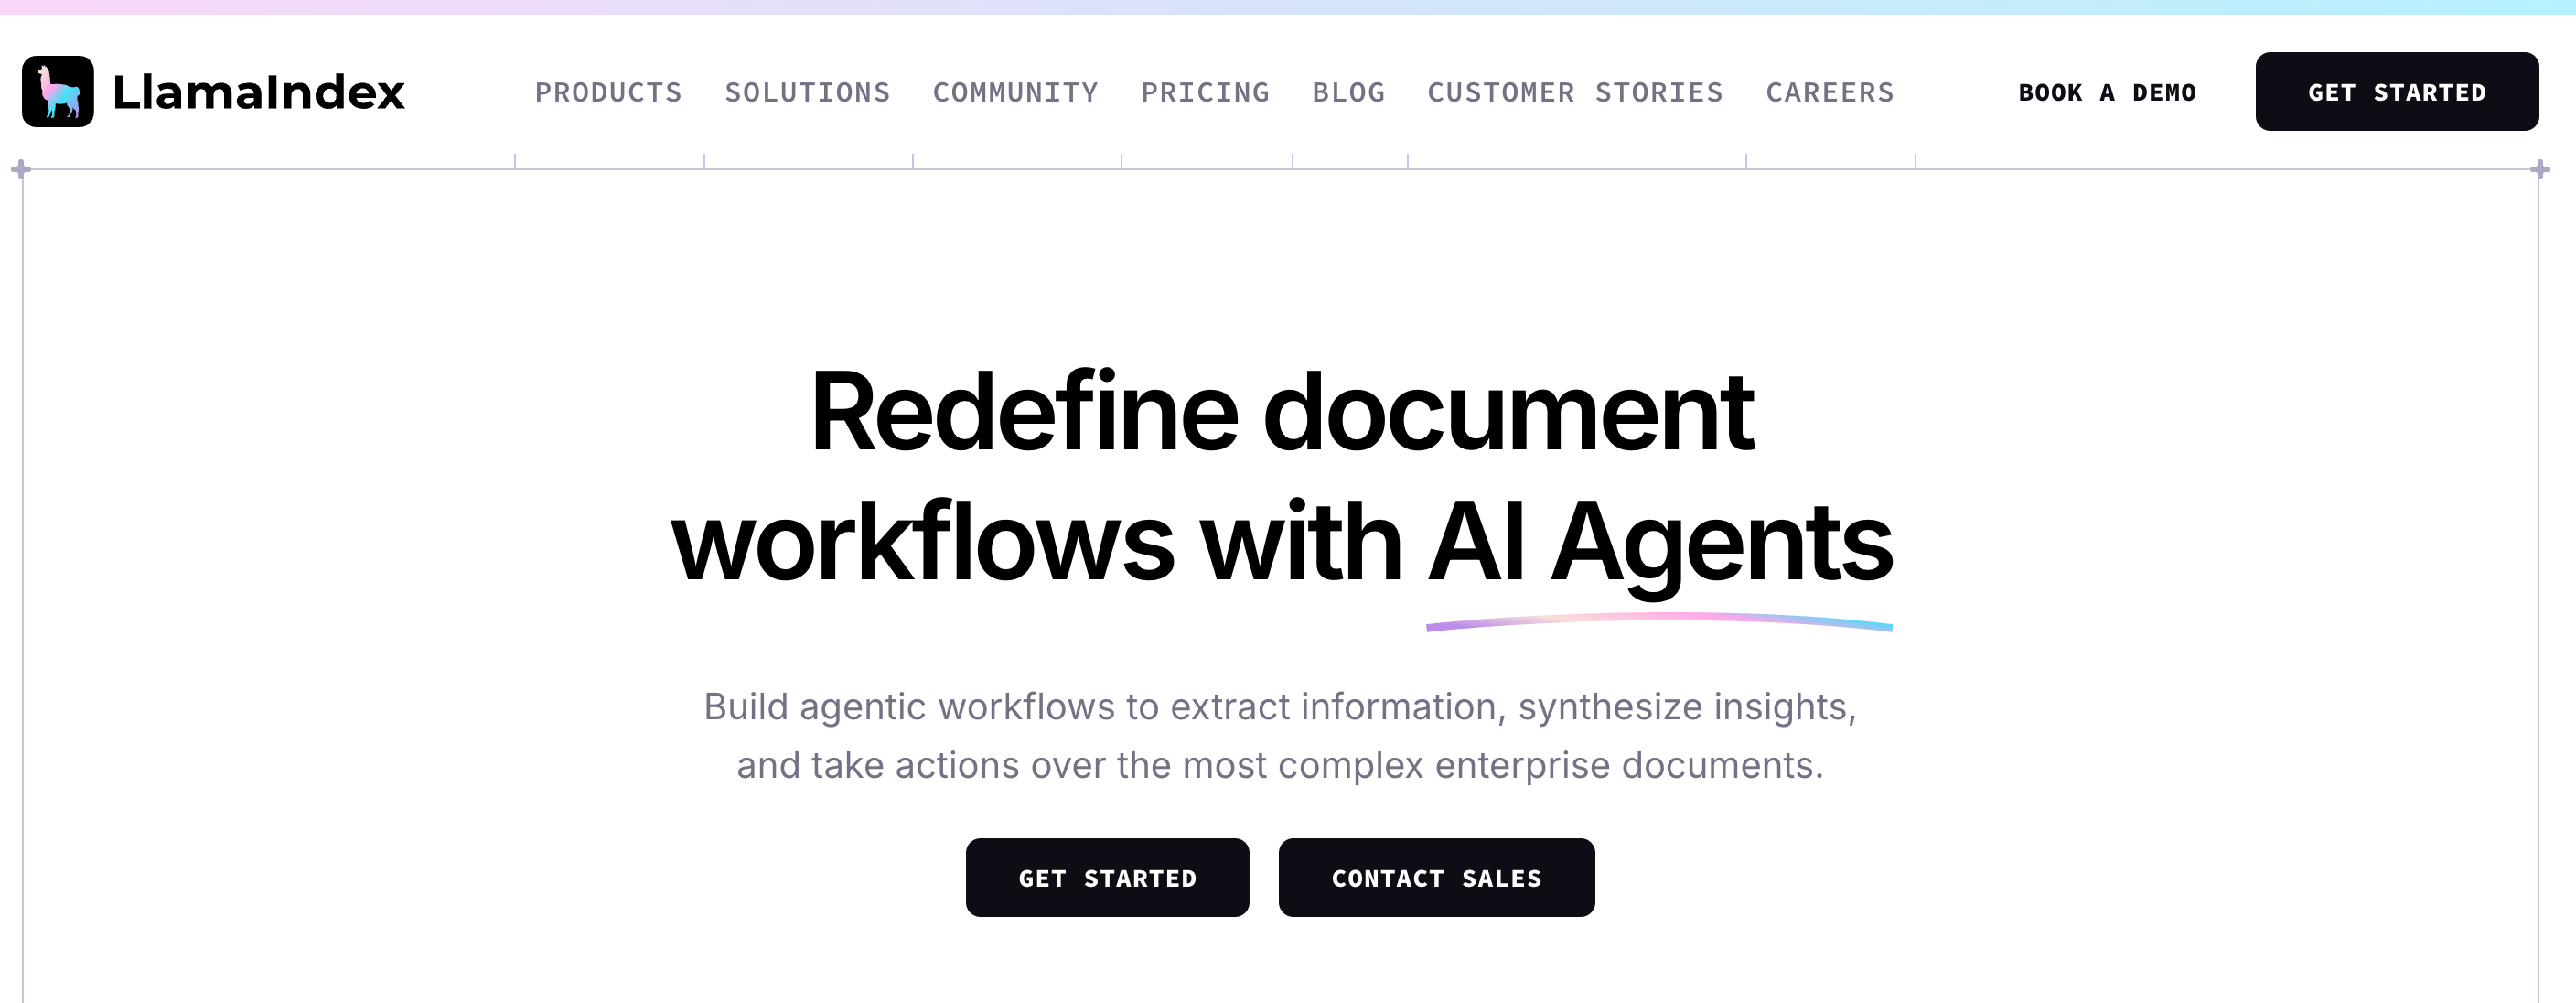
\includegraphics[width=0.8\linewidth,keepaspectratio]{aiagents58}
		
		{\tiny (Ref: Vizuara AI Agents Bootcamp)}
		
		\end{center}	
    \end{column}
  \end{columns}
\end{frame}

%%%%%%%%%%%%%%%%%%%%%%%%%%%%%%%%%%%%%%%%%%%%%%%%%%%%%%%%%%%
\begin{frame}[fragile]\frametitle{LlamaIndex: Unique Features}
\begin{columns}
    \begin{column}[T]{0.6\linewidth}
      \begin{itemize}
		\item Clear Workflow System: Structured agent pipelines with state management
		\item LlamaParse: GenAI-native document parsing for PDFs and complex files
		\item LlamaHub Tools: Ready-to-use connectors for Google Drive, Slack, search engines
		\item Plug-and-Play Components: Lego-like assembly of vector stores and LLM connectors
		\item Advanced Document Processing: Intelligent parsing for optimal LLM consumption
		\item One-Stop Framework: Complete toolkit beyond just retrieval or prompting
	  \end{itemize}
    \end{column}
    \begin{column}[T]{0.4\linewidth}
		\begin{center}
		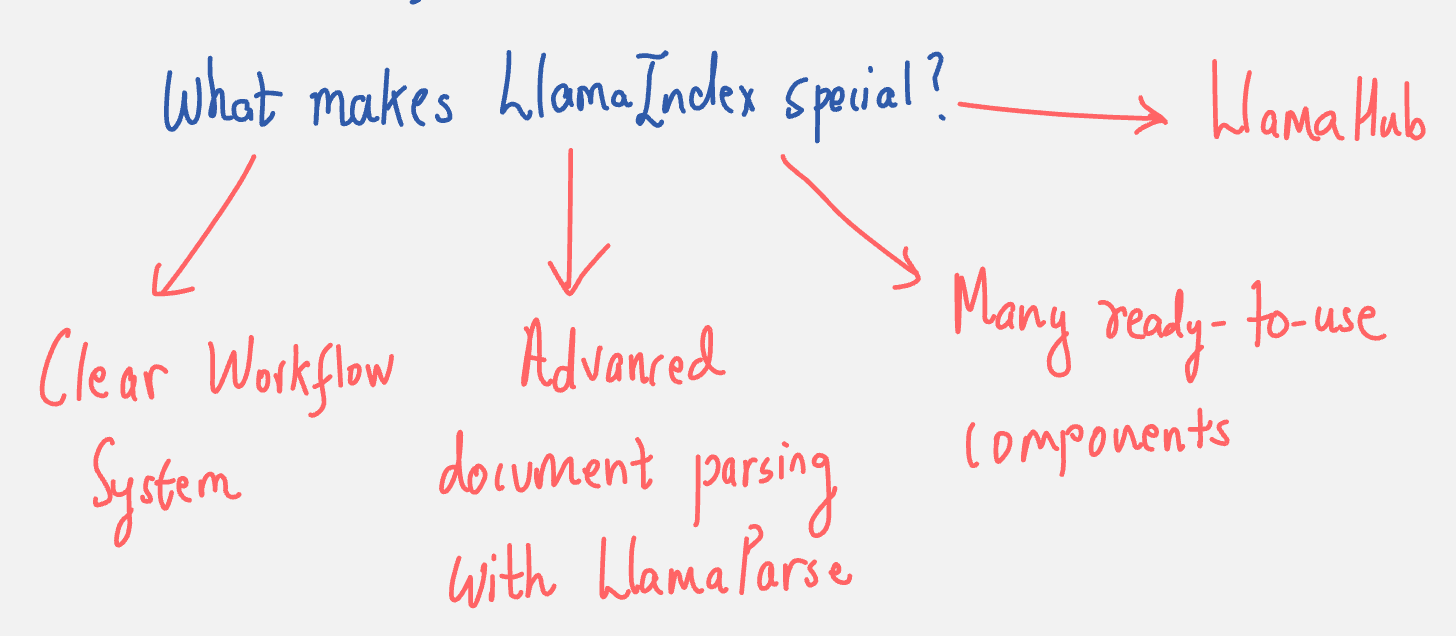
\includegraphics[width=0.8\linewidth,keepaspectratio]{aiagents59}
		
		{\tiny (Ref: Vizuara AI Agents Bootcamp)}
		\end{center}	
    \end{column}
  \end{columns}
\end{frame}


%%%%%%%%%%%%%%%%%%%%%%%%%%%%%%%%%%%%%%%%%%%%%%%%%%%%%%%%%%%
\begin{frame}[fragile]\frametitle{Agentic RAG Implementation: Data Setup}

      \begin{itemize}
		\item Document Loading: SimpleDirectoryReader for PDF and text files
		\item Text Chunking: SentenceSplitter with configurable chunk sizes (1024 tokens)
		\item LLM Configuration: OpenAI GPT-3.5-turbo for reasoning and generation
		\item Embedding Setup: OpenAI text-embedding-ada-002 for vector similarity
		\item Multiple Index Creation: Vector index for specific facts, Summary index for overviews
		\item Query Engine Setup: Specialized engines for different retrieval strategies
	  \end{itemize}


\end{frame}

%%%%%%%%%%%%%%%%%%%%%%%%%%%%%%%%%%%%%%%%%%%%%%%%%%%%%%%%%%%
\begin{frame}[fragile]\frametitle{Step 1: Loading and Chunking Data}


		\begin{lstlisting}
from llama_index.core import SimpleDirectoryReader, SentenceSplitter

# Load the document
reader = SimpleDirectoryReader(input_files=["State_of_AI_2025.pdf"])
documents = reader.load_data()
print(f"Loaded {len(documents)} document(s).")

# Split document into nodes (chunks)
splitter = SentenceSplitter(chunk_size=1024)
nodes = splitter.get_nodes_from_documents(documents)
print(f"Produced {len(nodes)} text chunks.")
		\end{lstlisting}	

\end{frame}

%%%%%%%%%%%%%%%%%%%%%%%%%%%%%%%%%%%%%%%%%%%%%%%%%%%%%%%%%%%
\begin{frame}[fragile]\frametitle{Step 2: Configuring LLM and Embeddings}


		\begin{lstlisting}
from llama_index.core import Settings
from llama_index.llms.openai import OpenAI
from llama_index.embeddings.openai import OpenAIEmbedding

Settings.llm = OpenAI(model="gpt-3.5-turbo")
Settings.embed_model = OpenAIEmbedding(model="text-embedding-ada-002")
		\end{lstlisting}	

\end{frame}


%%%%%%%%%%%%%%%%%%%%%%%%%%%%%%%%%%%%%%%%%%%%%%%%%%%%%%%%%%%
\begin{frame}[fragile]\frametitle{Step 3: Creating Multiple Indexes}


		\begin{lstlisting}
from llama_index.core import VectorStoreIndex, SummaryIndex

# Create a summary index (for high-level overview)
summary_index = SummaryIndex(nodes)

# Create a vector store index (for semantic search)
vector_index = VectorStoreIndex(nodes)
		\end{lstlisting}	

\end{frame}

%%%%%%%%%%%%%%%%%%%%%%%%%%%%%%%%%%%%%%%%%%%%%%%%%%%%%%%%%%%
\begin{frame}[fragile]\frametitle{Step 4: Building Query Engines}


		\begin{lstlisting}
# Create a query engine for each index
summary_query_engine = summary_index.as_query_engine(response_mode="tree_summarize")
vector_query_engine = vector_index.as_query_engine()
		\end{lstlisting}	

\end{frame}

%%%%%%%%%%%%%%%%%%%%%%%%%%%%%%%%%%%%%%%%%%%%%%%%%%%%%%%%%%%
\begin{frame}[fragile]\frametitle{Step 5: Wrapping Query Engines as Tools}


		\begin{lstlisting}
from llama_index.core.tools import QueryEngineTool

# Create tool interfaces for each query engine
summary_tool = QueryEngineTool.from_defaults(
    query_engine=summary_query_engine,
    description="Useful for summarizing the State of AI 2025 report."
)
vector_tool = QueryEngineTool.from_defaults(
    query_engine=vector_query_engine,
    description="Useful for retrieving specific details from the State of AI 2025 report."
)
		\end{lstlisting}	

\end{frame}

%%%%%%%%%%%%%%%%%%%%%%%%%%%%%%%%%%%%%%%%%%%%%%%%%%%%%%%%%%%
\begin{frame}[fragile]\frametitle{Step 6: Setting Up a Router Query Engine}


		\begin{lstlisting}
from llama_index.core.query_engine.router_query_engine import RouterQueryEngine
from llama_index.core.selectors import LLMSingleSelector

# Create a router that can select between the two query engine tools
router_engine = RouterQueryEngine(
    selector=LLMSingleSelector.from_defaults(),
    query_engine_tools=[summary_tool, vector_tool],
    verbose=True
)

response = router_engine.query("Who is Lareina Yee according to the document?")
print(response)
# (It should retrieve context and answer that Lareina Yee is one of the authors.)
		\end{lstlisting}	

\end{frame}



%%%%%%%%%%%%%%%%%%%%%%%%%%%%%%%%%%%%%%%%%%%%%%%%%%%%%%%%%%%
\begin{frame}[fragile]\frametitle{Tool Creation and Agent Setup}

      \begin{itemize}
		\item QueryEngineTool Wrapping: Convert query engines into agent-usable tools
		\item Tool Descriptions: Clear descriptions help agent choose appropriate tool
		\item RouterQueryEngine: Automated routing between summary and vector tools
		\item LLMSingleSelector: Intelligent tool selection based on query analysis
		\item AgentWorkflow: High-level API for creating agents with tool access
		\item System Prompts: Context-aware prompts for specialized agent behavior
	  \end{itemize}
  
\end{frame}

%%%%%%%%%%%%%%%%%%%%%%%%%%%%%%%%%%%%%%%%%%%%%%%%%%%%%%%%%%%
\begin{frame}[fragile]\frametitle{Step 7: Defining the Agent}


		\begin{lstlisting}
from llama_index.core.agent.workflow import AgentWorkflow

# Wrap the router query engine as a tool for the agent
assistant_tool = QueryEngineTool.from_defaults(
    query_engine=router_engine,
    name="state_of_ai_report_assistant",
    description="Tool to answer questions using the McKinsey 2025 State of AI report."
)

# Initialize the agent with this tool
agent = AgentWorkflow.from_tools_or_functions(
    tools_or_functions=[assistant_tool],
    llm=Settings.llm,
    system_prompt="You are an AI assistant skilled in answering questions about the 2025 State of AI report."
)
		\end{lstlisting}	

\end{frame}

%%%%%%%%%%%%%%%%%%%%%%%%%%%%%%%%%%%%%%%%%%%%%%%%%%%%%%%%%%%
\begin{frame}[fragile]\frametitle{Step 8: Running the Agent}


		\begin{lstlisting}
# Ask the agent a complex question
question = "Summarize the key trends in AI adoption and mention the percentage of companies using AI."
response = await agent.run(question)
print(response)
		\end{lstlisting}	

\end{frame}
